\subsection{Cloud Computing Modelle}

\begin{figure}[h]
    \centering
    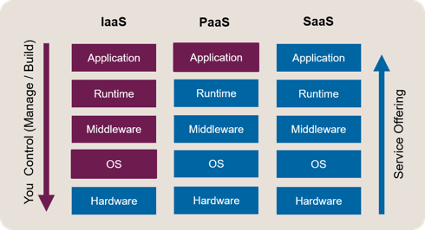
\includegraphics[scale=0.9]{sections/cloud-computing/images/models.png}
    \caption{Modelle}
\end{figure}

\subsubsection{Infrastructure as a Service (IaaS)}

Infrastructure as a Service stellt sowohl virtuelle und physische Server, als auch Netzwerk- und Speicherressourcen, nach Verlangen des Verbrauchers, zur Verfügung. Der Nutzer hat die völlige Kontrolle über Ressourcen, in Bezug auf Speicher und Rechenleistung. Die Auswahl des Betriebssystems wird ebenfalls dem Nutzer überlassen. Beispiele hierfür sind Amazon EC2-Cluster und Microsoft Azure.

\subsubsection{Platform as a Service (PaaS)}

Diese Form des Cloud Computing gibt dem Kunden die Möglichkeit, seine Anwendungen auf einer, vom Dienstleistungsgeber, gehosteten Plattform zu entwickeln, bereitzustellen und zu verwalten. Bei diesem Modell handhabt der Dienstleister sämtliche Ressourcen. Die Anwendung wird den potenziellen Nutzern über APIs zur Verfügung gestellt. Hierbei ist wichtig, dass der Nutzer keinerlei Einfluss über, die im Hintergrund laufenden, Ressourcen hat. Bekannte Beispiele hierfür sind Web-Hosting Dienste, wie etwa +Microsoft Azure Web und Amazon Web Services.

\subsubsection{Software as a Service (SaaS)}

Bei SaaS wird den Nutzern die Möglichkeit gegeben auf eine, vom Dienstleister in der Cloud Infrastruktur bereitgestellten Anwendung, zu zugreifen und zu benutzen. Benutzer können dann über eine webbasierte Schnittstelle, wie beispielsweise ftp und clientseitige Schnittstellen, darauf zugreifen. Jene Anwendungen werden gegen monatliche oder jährliche Zahlungen dem Benutzer bereitgestellt. Jedoch hat der Verbraucher keine bis wenig Kontrolle über im Hintergrund geregelte Ressourcen. Beispiele hierfür sind Microsoft Office 365, Microsoft Skype und Google Apps.